\documentclass[twocolumn,10pt,a4paper]{article}
\usepackage[margin=0.75in]{geometry}
\usepackage[utf8]{inputenc}
\usepackage[T1]{fontenc}
\usepackage{lmodern}
\usepackage{microtype}
\usepackage{cite}
\usepackage{url}
\usepackage{hyperref}
\usepackage{xcolor}
\usepackage{enumitem}
\usepackage{tabularx}
\usepackage{booktabs}
\usepackage{graphicx}
\hypersetup{colorlinks=true,citecolor=blue,linkcolor=blue,urlcolor=blue}

\title{Paper 4: Structural Communication Safety Boundary for Deterministic O-RAN Authorization}

\author{David Kypuros \\
\small Red Hat \\
\small \texttt{dkypuros@redhat.com}}

\date{2 June 2026}

\begin{document}
\maketitle

\begin{abstract}
Paper 4 in this five-paper series describes the structural communication boundary used by the O-RAN Agent Harness to contain nondeterminism in Cloud RAN remediation. The harness does not let an LLM generate raw configuration, shell commands, direct REST calls, or live hardware mutations. Its first decision point is deterministic: a taxonomy-backed router classifies the fault and selects the service route, infrastructure route, or ambiguous class before any LLM is consulted. The LLM is only a support mechanism for ambiguous cases. Every proposed action must then pass a schema gate, a five-subcheck policy guardrail, and human co-authorization before it can be represented as a standards-shaped TMF688, TMF921, or O2 IMS handoff. The contribution of this paper is the structural communication boundary: nondeterministic reasoning can assist diagnosis, but execution authority is carried only by validated structures, policy results, audit records, and operator approval.
\end{abstract}

\section{Introduction}

The integration of agentic AI into telecom operations represents a fundamental shift in how networks are managed. A prior multivendor diagnostic publication demonstrated the efficacy of agents in root-cause localization across timing, RAN, and platform domains \cite{multivendor_blog_2026}. However, diagnosis is fundamentally an observation problem; remediation is a mutation problem. When an agent transitions from analyzing a fault payload to proposing a concrete physical change---such as a host reboot, firmware update, or driver swap---the tolerance for hallucination drops to zero.

The operational problem is not merely identifying the correct action, but safely translating a fault-driven remediation proposal into a physical or service-affecting change without allowing AI-generated text to become execution authority. In a multivendor O-RAN deployment, the executing environment is governed by strict standards \cite{oran_wg1_arch,oran_o2_ganp} and controlled by rigid operator contracts \cite{openshift_mco,metal3_bmo}. Exposing these critical execution surfaces directly to an LLM is both technologically unsafe and operationally unacceptable.

This paper outlines the O-RAN Agent Harness's solution to this problem: structural demarcation. Section \ref{sec:demarcation} explains the boundary between cognitive assistance and deterministic execution. Section \ref{sec:containment} details the schema-driven containment strategy and the deterministic taxonomy/router. Section \ref{sec:gates} describes the schema gate, five-subcheck policy guardrail, and human co-authorization chain. Section \ref{sec:handoffs} maps the output to standards-shaped TM Forum and O-RAN envelopes. Section \ref{sec:discuss} contextualizes this approach within the broader telecom landscape. Section \ref{sec:limits} states the v0 evidence boundary, and Section \ref{sec:conclude} concludes.

\section{The Principle of Structural Demarcation}
\label{sec:demarcation}

The Agent Harness architecture enforces a strict separation of concerns between observation, cognitive assistance, routing, and execution. The deterministic taxonomy/router is the first-class decision point: it maps incoming telemetry signals, including O-RAN Cloud Notifications envelopes \cite{oran_cloud_notifications}, onto harness-defined taxonomy classes and route types. The LLM has no direct write authority over the plant and is not the primary router. It is consulted only when the deterministic router returns the \texttt{ambiguous} class.

\begin{figure*}[t]
\centering
\vspace{1em}
\includegraphics[width=\textwidth]{../talk/architecture.png}
\vspace{1em}
\caption{Seven-component macro architecture. The deterministic router and governance layer bound any LLM influence: non-ambiguous cases route without an LLM, ambiguous cases may receive LLM support, and no proposal crosses the execution boundary without validated structure, policy approval, and human co-authorization.}
\label{fig:arch_macro}
\end{figure*}

By forcing all remediation state through strict schemas such as \texttt{RCA.json} and \texttt{RemediationProposal.json}, the harness converts diagnostic output into a predictable, strongly typed artifact. The agent runtime does not execute commands; it produces candidate structure. The environment does not trust prose, model confidence, or free-form instructions. It accepts only schema-valid fields, deterministic route classes, policy outcomes, and operator decisions.

\section{Cognitive Containment via Schemas}
\label{sec:containment}

When the diagnostic agent evaluates a fault, it is not permitted to generate free-form text or direct API invocations. Instead, it must draft a formal remediation proposal. The structure of this proposal is dictated by a strict JSON Schema definition.

A valid remediation proposal requires several deterministic elements. It must provide a \texttt{taxonomyMatch} that is cleanly grounded in the O-RAN Working Group 6 resource model \cite{oran_o2_ganp}. It must specify an \texttt{actionType} (e.g., applying a MachineConfig or executing a bare-metal firmware write) and name the precise \texttt{actionTarget} within the cluster topology.

This rigid structure ensures that if the LLM hallucinates an invalid target, invents an unknown taxonomy class, or attempts a malformed action sequence, the resulting payload will fail to conform to the schema. The schema validation engine traps and aborts the hallucination long before it approaches the network's execution boundaries.

\section{Schema Gate, Policy Guardrail, and Human Co-Authorization}
\label{sec:gates}

Before any structural proposal is allowed to leave the remediation boundary, it must pass through three deterministic control points: a schema gate, a five-subcheck policy guardrail, and human co-authorization.

The \textbf{schema gate} validates the payload against the defined draft-07 JSON Schema. This step rejects malformed data types, missing required fields, unapproved enumerations, invalid taxonomy classes, and malformed remediation or reversibility-profile subobjects.

The \textbf{five-subcheck policy guardrail} is an LLM-free policy enforcement point. Its subchecks fire in order: \texttt{crisis\_mode} global override, sandbox \texttt{apply\_allowed}, \texttt{action\_allowlist}, \texttt{blast\_radius} caps, and \texttt{requiresHumanApproval}. The v0 blast-radius caps are intentionally narrow: one node, one site, and four cells. The v0 sandbox verdict is fixture-driven; production wiring would source the verdict from a mirrored cluster or equivalent simulation environment.

The final control point is \textbf{human co-authorization}. The operator receives the TMF688-shaped audit event, the sandbox verdict, the policy result, the optional TMF921-shaped companion intent and dispatch result, and the seven-field ReversibilityProfile before commit. In v0 this is a boolean approval boundary; proposal editing before commit is future work.

After such an \texttt{AuditEvent} exists, an LLM-backed chat assistant may summarize or explain the deterministic evidence for the operator. That post-event explanation does not change the taxonomy match, guardrail result, sandbox verdict, companion-intent outcome, or human approval state.

\section{Shape-Correct Standards Handoffs}
\label{sec:handoffs}

\begin{figure*}[t]
\centering
\vspace{1em}
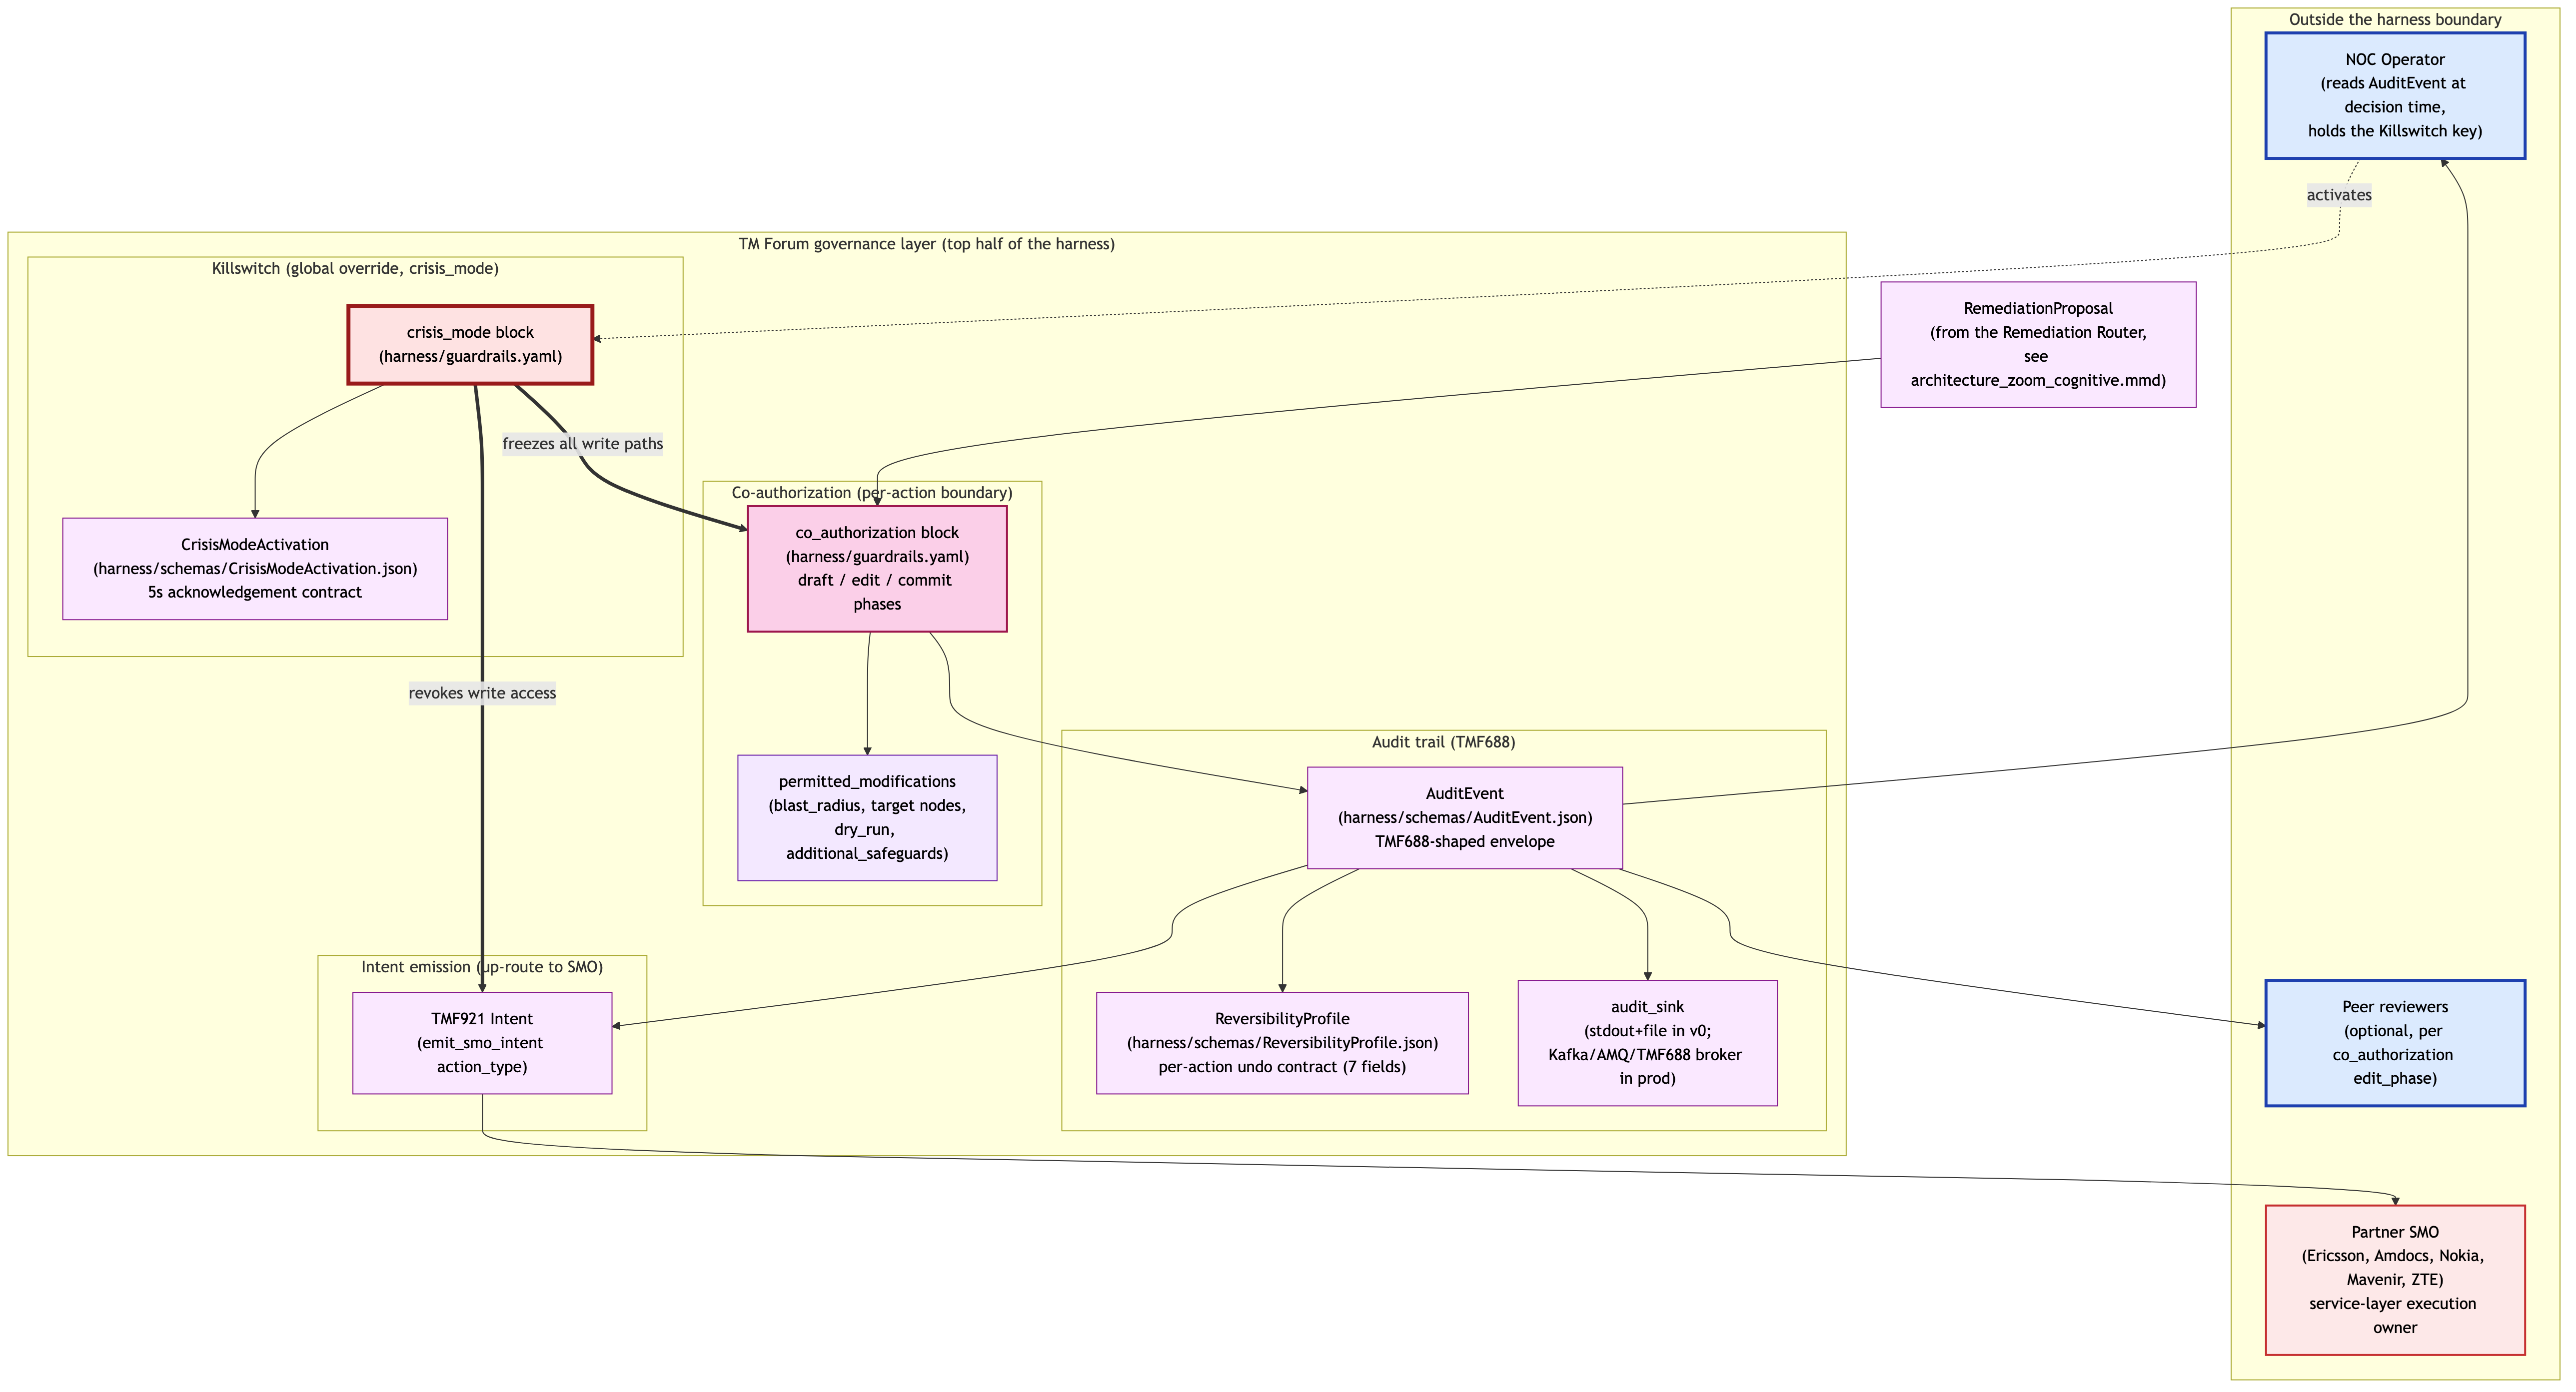
\includegraphics[width=\textwidth]{../talk/architecture_zoom_governance.png}
\vspace{1em}
\caption{Governance layer zoom. The proposals that survive the twin gates are formatted into standard TMF688 audit envelopes, exposing the reversibility profile and the O2 IMS dispatch structures to the human operator for final authorization.}
\label{fig:governance}
\end{figure*}

To maintain trust without overstating maturity, the harness shapes its decisions into established telecom envelopes. These are standards-shaped handoffs, not claims of live standards-body interop. The architecture deliberately avoids proprietary execution channels while acknowledging that v0 uses fixture replay and stubbed boundaries.

\textbf{TM Forum TMF688 (Event Management API):} All human review requests, sandbox verdicts, and governance logs are formatted as TMF688 \texttt{AuditEvent} envelopes \cite{tmf688}. This structure embeds a seven-field Reversibility Profile, ensuring the operational evidence chain integrates seamlessly with standard enterprise observability streams.

\textbf{TM Forum TMF921 (Intent Management API):} When an infrastructure action requires service-layer coordination---such as requesting a maintenance window before an intrusive reboot---the harness issues a TMF921-shaped companion intent upward to the partner SMO \cite{tmf921, oran_decoupled_smo}.

\textbf{O-RAN O2 IMS-shaped boundary:} Infrastructure remediation directives are represented as O2 IMS-shaped payloads and routed downward to a v0 O-Cloud Manager stub boundary \cite{oran_o2_ims, oran_o2ims_ocm}. The v0 evidence is a shape-correct \texttt{o2ims\_dispatch} envelope plus CRD-shaped fixtures, not live O2 IMS interop.

\section{Execution Delegation to Native Reconcilers}
\label{sec:delegation}

The risk-reducing discipline of the structural communication model is \textbf{execution delegation}. The Agent Harness itself is not the live mutation engine for infrastructure.

Once the operator co-authorizes a valid \texttt{RemediationProposal}, the v0 O-Cloud Manager stub records the intended O2 IMS-shaped dispatch and points to committed Kubernetes CRD-shaped fixtures. In production, the corresponding execution would be delegated to native reconcilers rather than performed by the harness. Host OS configurations map to the Machine Config Operator (MCO) \cite{openshift_mco}; out-of-tree driver swaps map to Kernel Module Management (KMM) \cite{kmm_operator}; and out-of-band firmware updates map to the Metal3 BareMetal Operator (BMO) using DMTF Redfish \cite{metal3_bmo, dmtf_redfish}. The safety claim is not that v0 performs live reconciliation, but that execution authority terminates at structural contracts and trusted reconcilers rather than at LLM output.

\section{Discussion}
\label{sec:discuss}

The structural communication pattern described here is highly complementary to orchestration platforms like Nephio \cite{nephio} and ONAP \cite{onap}. While those systems excel at managing the standing topology and lifecycle of network functions, the Agent Harness addresses post-deployment, anomaly-driven Day-2 remediation.

A common criticism of AI-driven automation is the lack of determinism and accountability. The schema gate, five-subcheck policy guardrail, standards-shaped handoffs, and human co-authorization boundary directly address these concerns. The key design point is ordering: deterministic taxonomy routing happens first, and LLM support is limited to ambiguous cases. The human operator remains the execution authority, with the audit event carrying the evidence needed to approve, reject, or defer the proposed change.

The live lab chat path is therefore an explanation surface, not an authority surface. It can read scoped slash-command outputs and a harness-walker sidecar, but it cannot turn prose into a routed or approved production mutation.

\section{Honest Scope}
\label{sec:limits}

The v0 claim is deliberately bounded. The harness demonstrates schema-gated proposal flow, a five-subcheck policy guardrail, human co-authorization, TMF688/TMF921-shaped records, an O2 IMS-shaped stub boundary, and CRD-shaped fixtures. It does not prove live O2 IMS interoperability, live TMF921 exchange, live Redfish writes, live Kubernetes reconciler commits, or standards-body conformance for the harness-authored schemas. Those are v1 interop and validation targets, not v0 claims.

\section{Conclusion}
\label{sec:conclude}

Closed-loop remediation in an O-RAN Cloud RAN environment cannot safely rely on autonomous AI acting directly on physical infrastructure. This paper has argued for structural demarcation instead: observe through standards-shaped envelopes, classify through a deterministic taxonomy/router, allow LLM support only for ambiguous cases, and pass every proposed mutation through a schema gate, five-subcheck policy guardrail, and human co-authorization. The v0 harness demonstrates this boundary with fixture replay, an O2 IMS-shaped stub boundary, TMF688/TMF921-shaped records, and CRD-shaped fixtures rather than live interop. This structural communication model provides a safer blueprint for operationalizing generative AI near critical cyber-physical telecom systems without making the model itself an execution authority.

\section*{Acknowledgements}

This paper builds upon a prior multivendor diagnostic substrate co-authored with S. Kiani Mehr, N. Korati Prasanna, M. Vazquez Cebrian, S. Srikanthan, and P. Venkatesh \cite{multivendor_blog_2026}. Source code is Apache-2.0 licensed and available at \url{https://github.com/dkypuros/oran-agent-harness}.

\bibliographystyle{plain}
\bibliography{refs}

\end{document}
